\documentclass[a4paper]{article}
\usepackage[14pt]{extsizes}
\usepackage[utf8]{inputenc}
\usepackage[russian]{babel}
\usepackage{setspace,amsmath}
\usepackage{graphicx}
\usepackage[font={small}]{caption}
\usepackage{color}
\usepackage[left=30mm, top=20mm, right=10mm, bottom=20mm, nohead, footskip=10mm]{geometry} 
\usepackage{indentfirst}
\parindent=1.25cm
\begin{document}
\section*{Влияние магнитного поля и шума на температурные профили}
\subsection*{Влияние магнитного поля}
\begin{figure}[h!]
\center{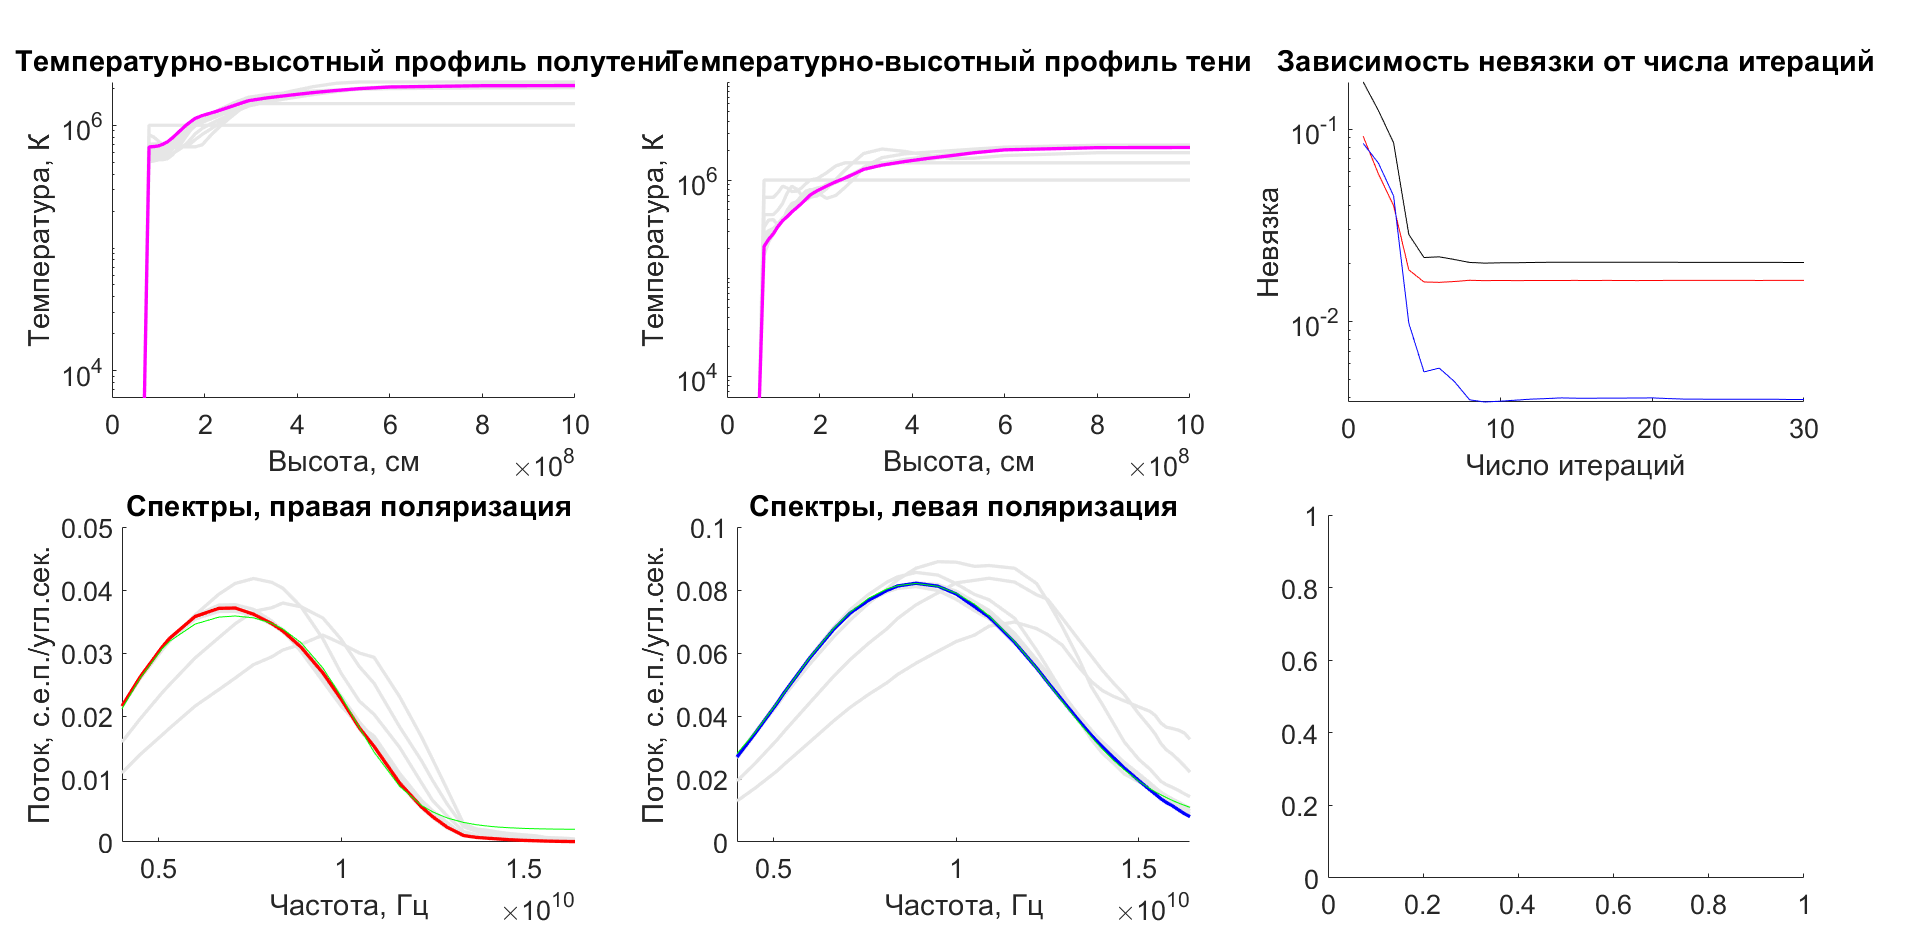
\includegraphics[width=1\linewidth]{FieldFactor/1.png}}
\caption{Поле увеличено на 1 процент}
\end{figure}
\begin{figure}[h!]
\center{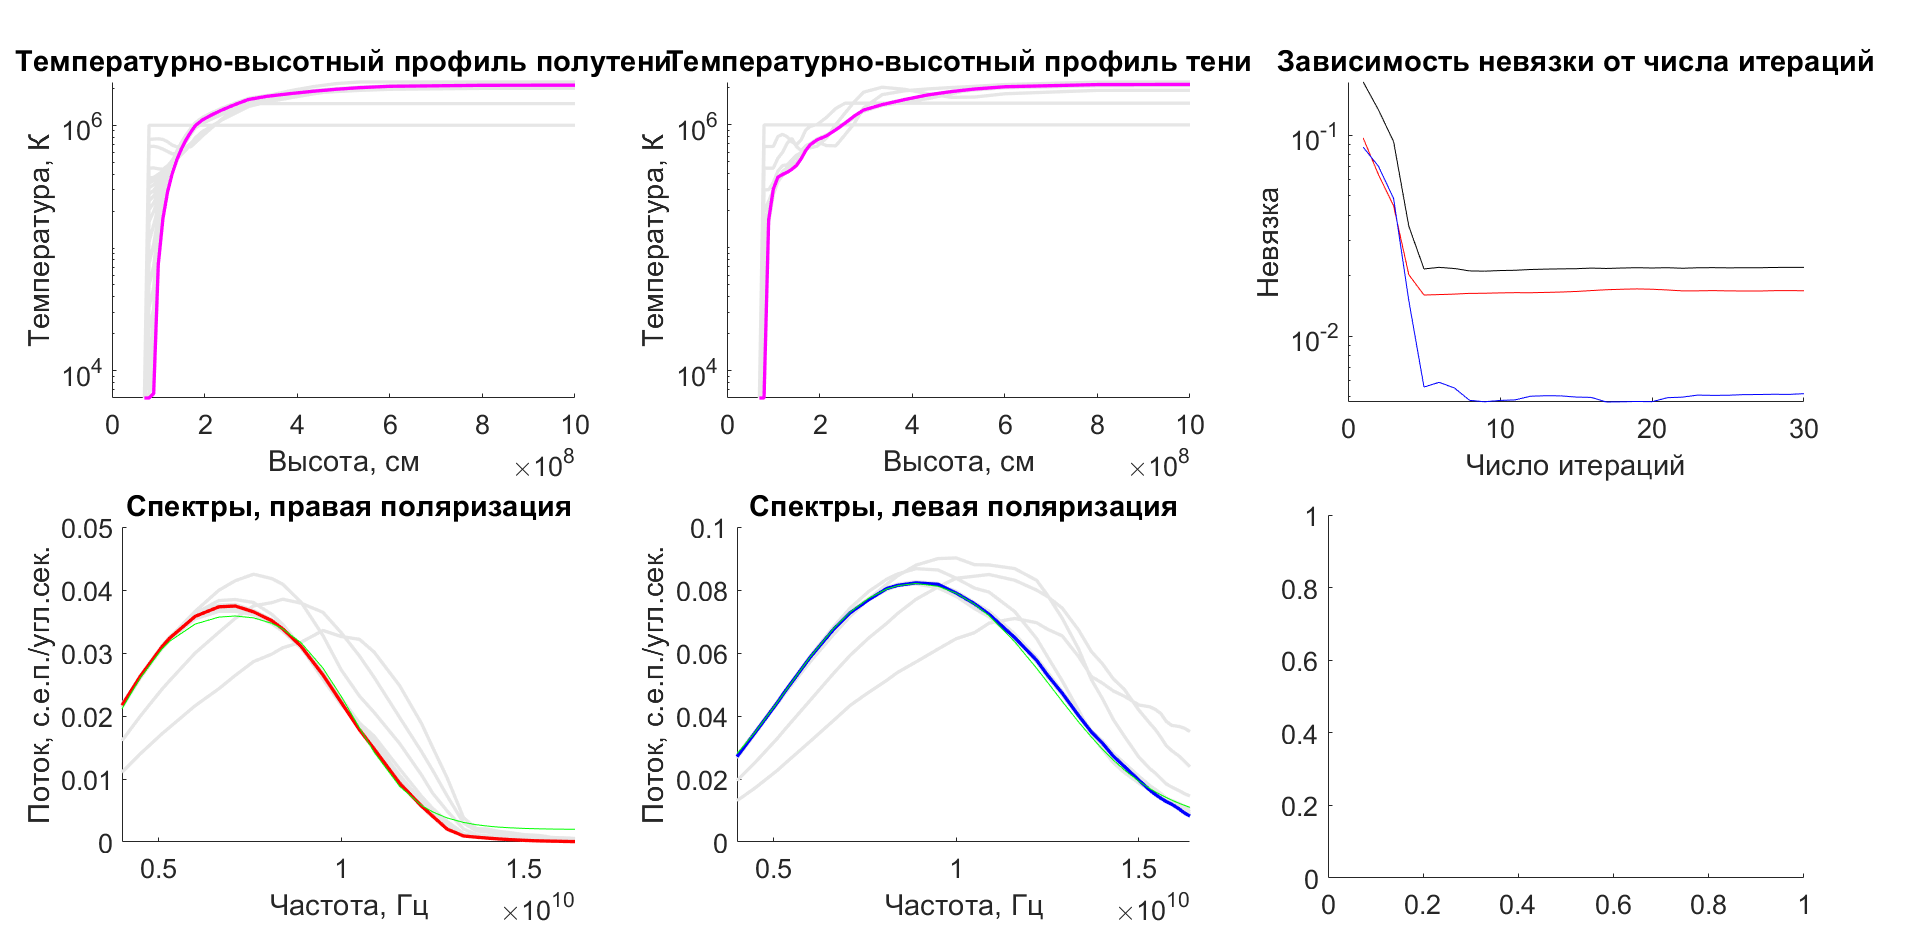
\includegraphics[width=1\linewidth]{FieldFactor/2.png}}
\caption{Поле увеличено на 2 процента}
\end{figure}
\begin{figure}[h!]
\center{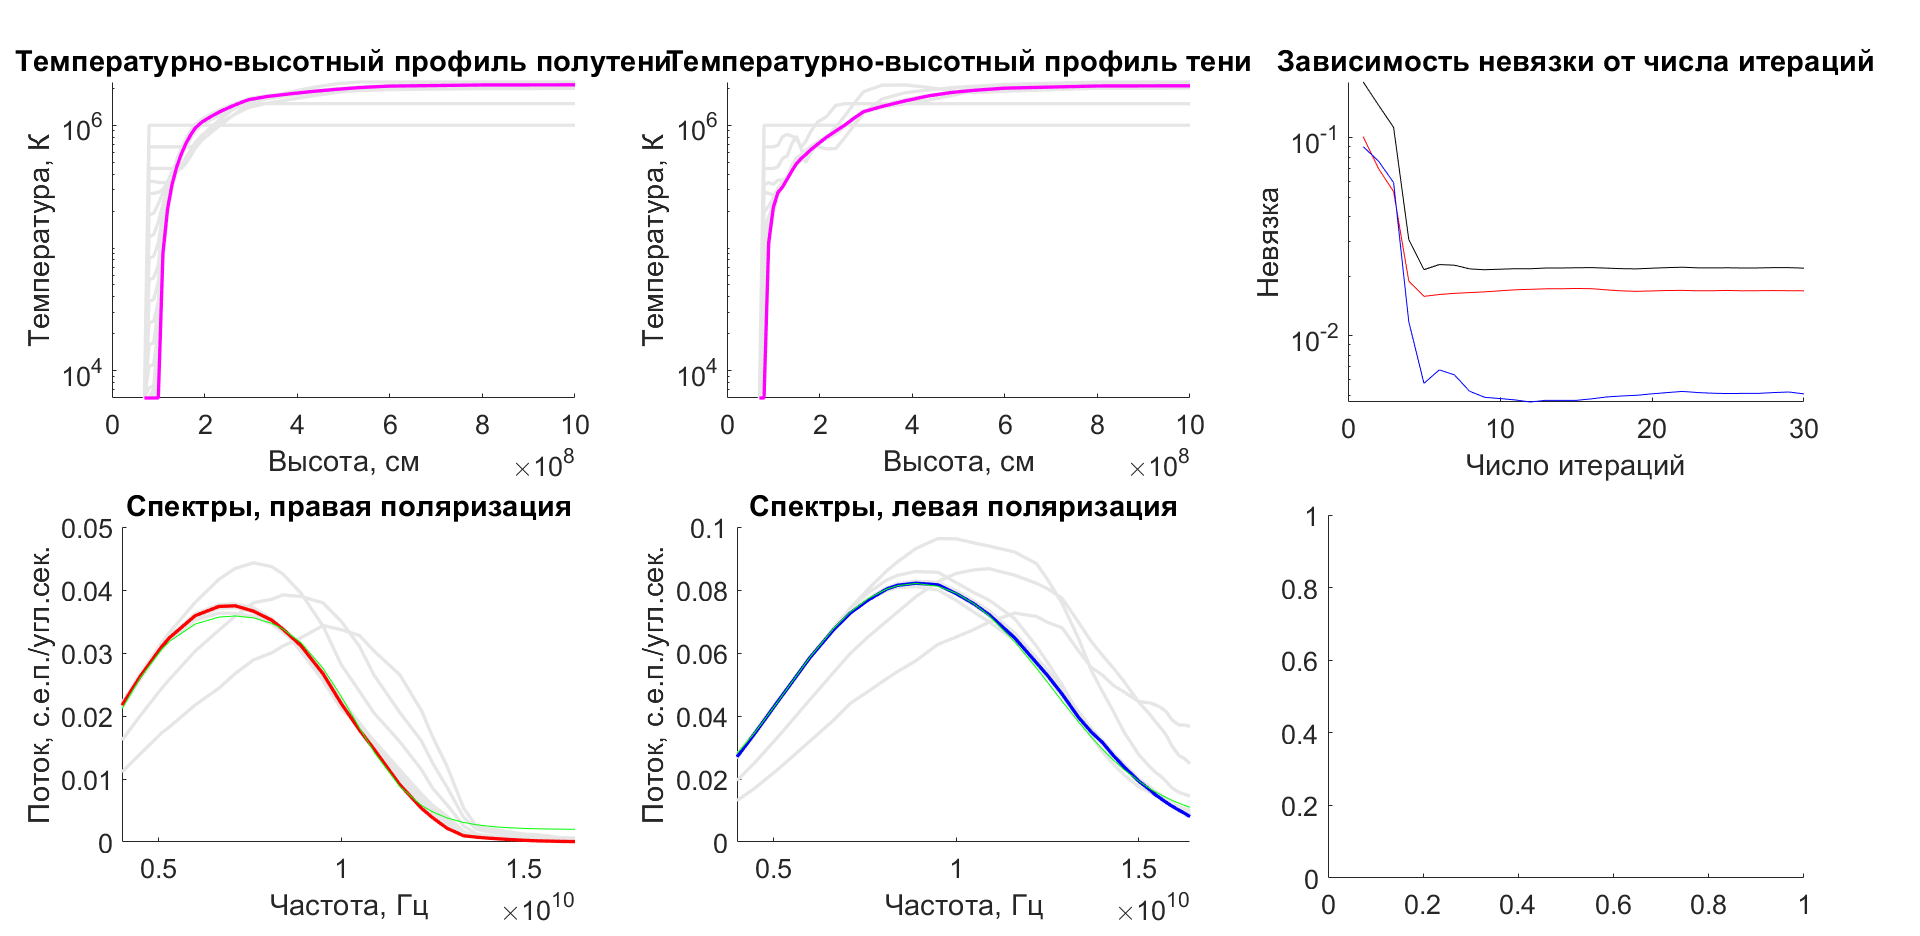
\includegraphics[width=1\linewidth]{FieldFactor/3.png}}
\caption{Поле увеличено на 3 процента}
\end{figure}
\begin{figure}[h!]
\center{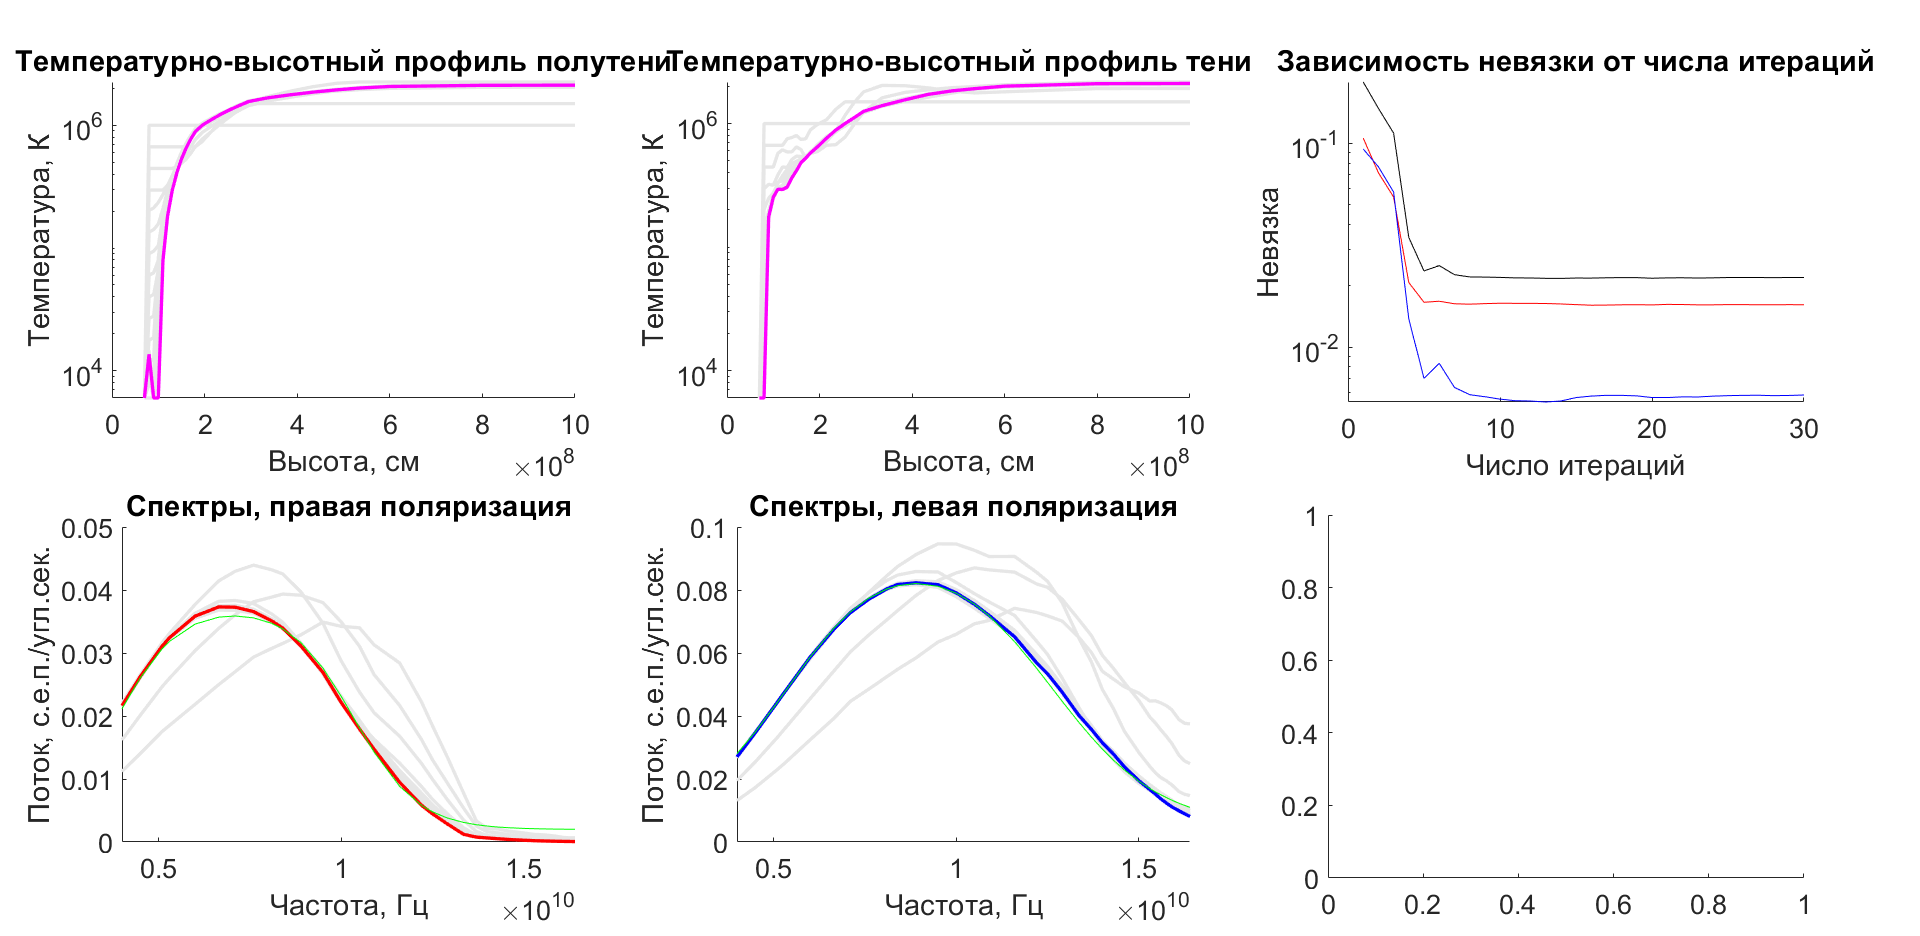
\includegraphics[width=1\linewidth]{FieldFactor/4.png}}
\caption{Поле увеличено на 4 процента}
\end{figure}
\begin{figure}[h!]
\center{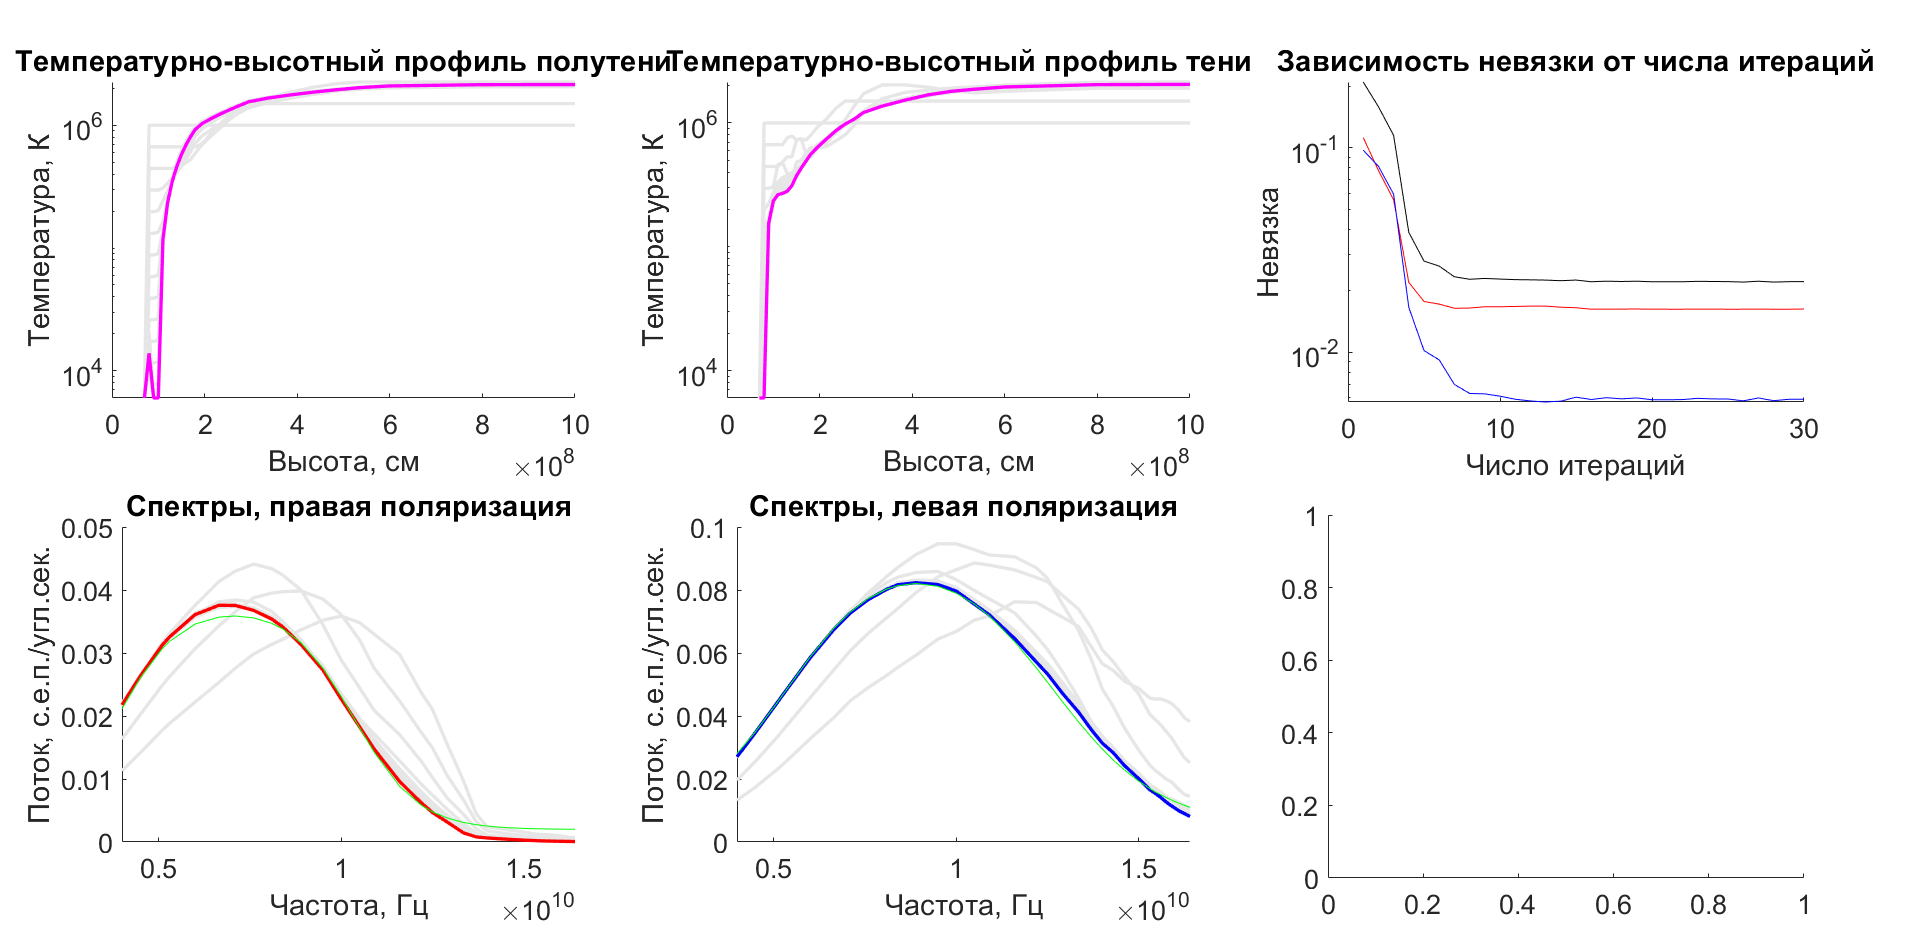
\includegraphics[width=1\linewidth]{FieldFactor/5.png}}
\caption{Поле увеличено на 5 процентов}
\end{figure}
\hfill\break
\hfill\break
\hfill\break
\hfill\break
\hfill\break
\hfill\break
\hfill\break
\hfill\break
\hfill\break
\hfill\break
\hfill\break
\hfill\break
\hfill\break
\hfill\break
\hfill\break
\hfill\break
Как видно из графиков, происходит сглаживание профилей в переходной области, но на 4 и 5 процентах появляется излом в начале профиля.
\newpage
\subsection*{Влияние аддитивного шума}
\begin{figure}[h!]
\center{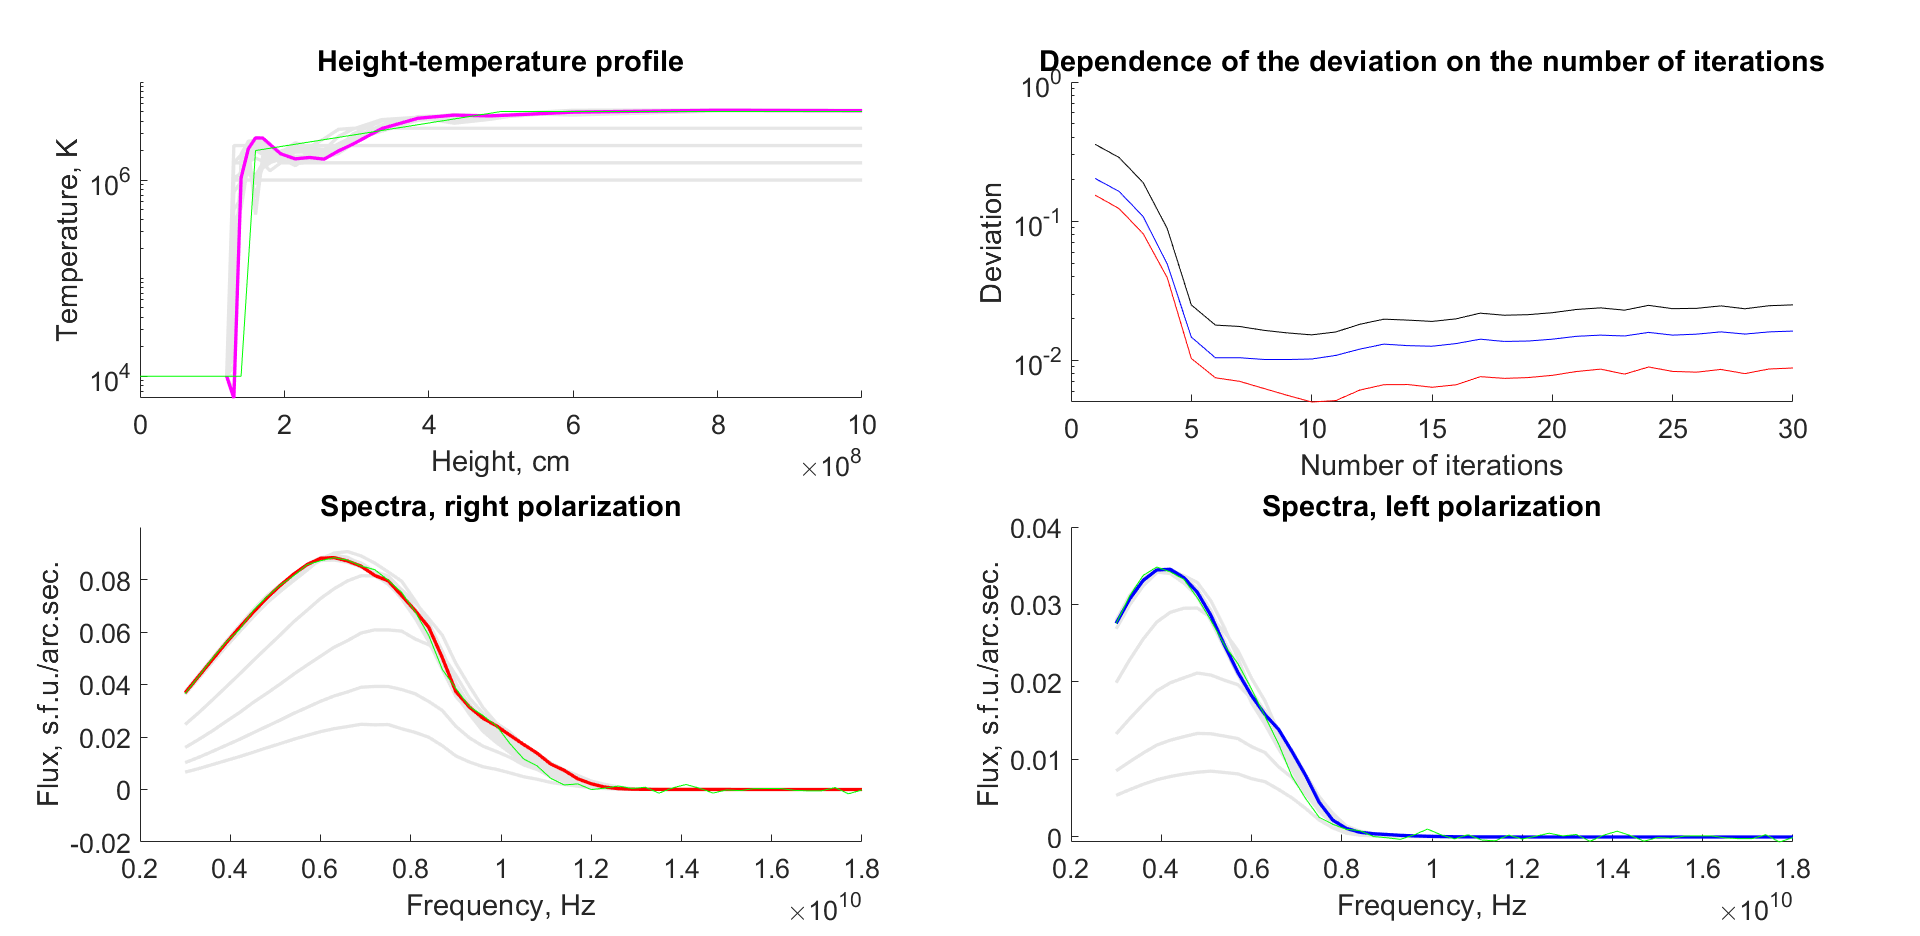
\includegraphics[width=1\linewidth]{AdditiveNoise/1.png}}
\caption{1-процентный аддитивный шум}
\end{figure}
\begin{figure}[h!]
\center{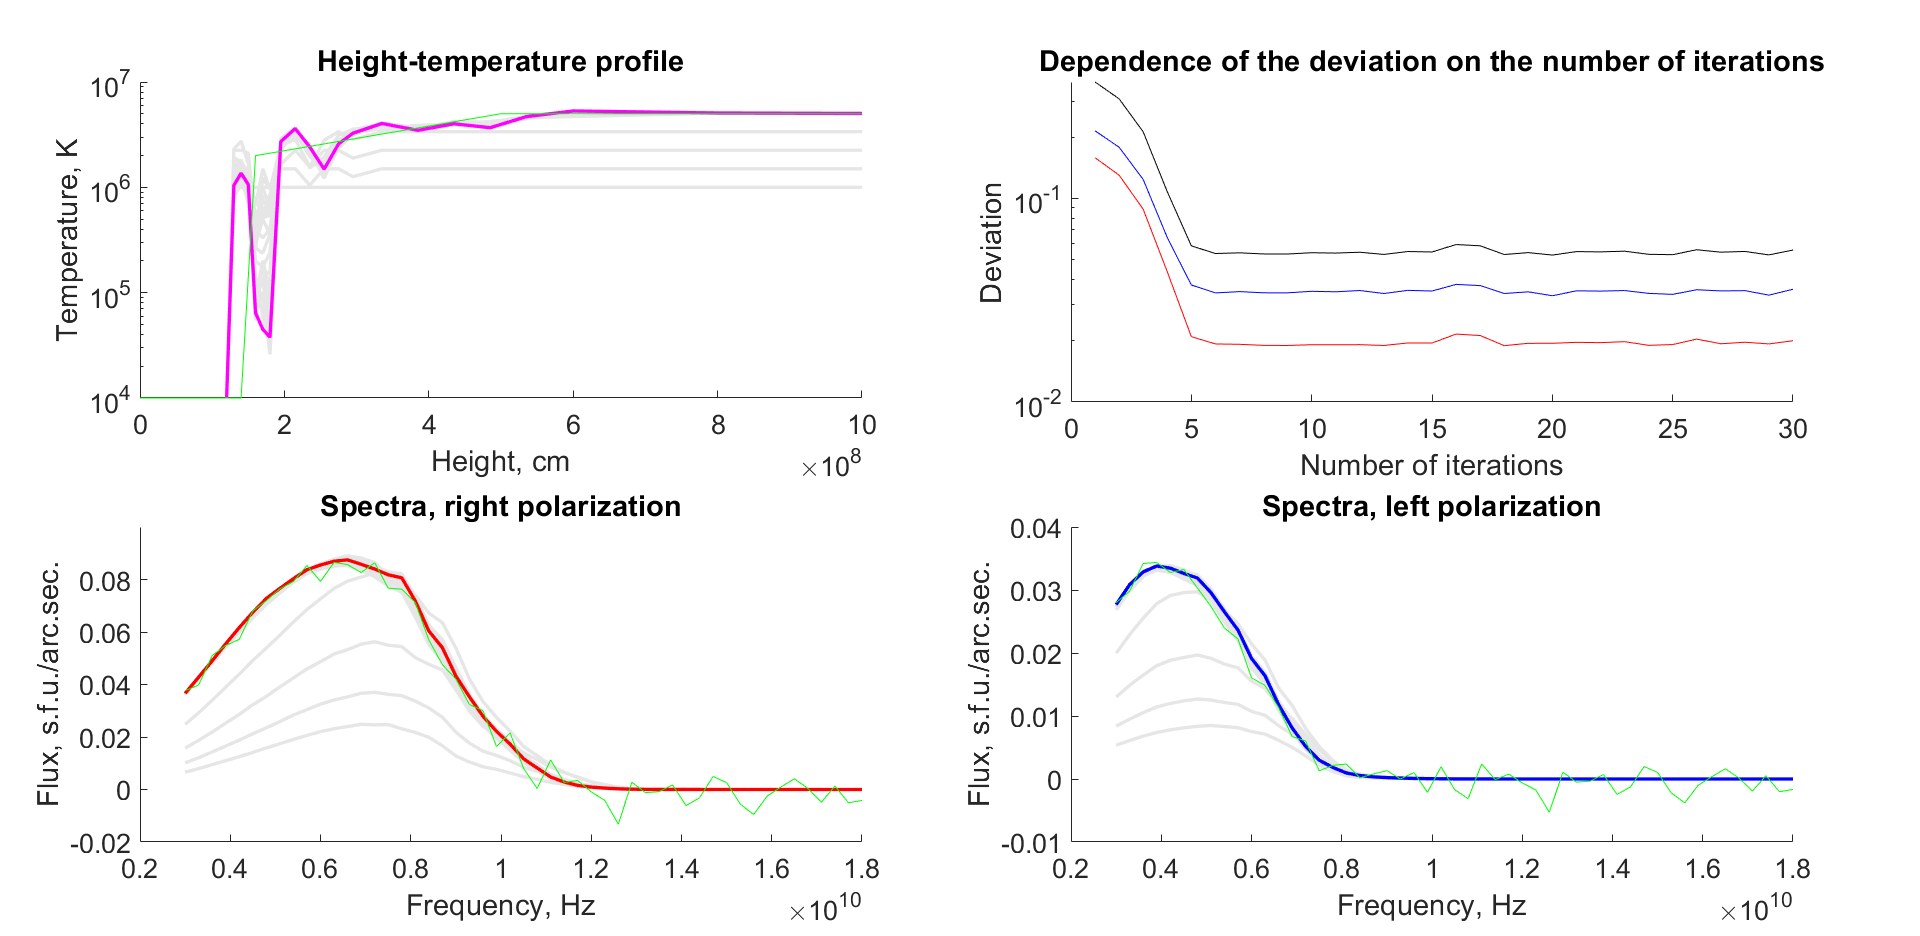
\includegraphics[width=1\linewidth]{AdditiveNoise/5.png}}
\caption{5-процентный аддитивный шум}
\end{figure}
\begin{figure}[h!]
\center{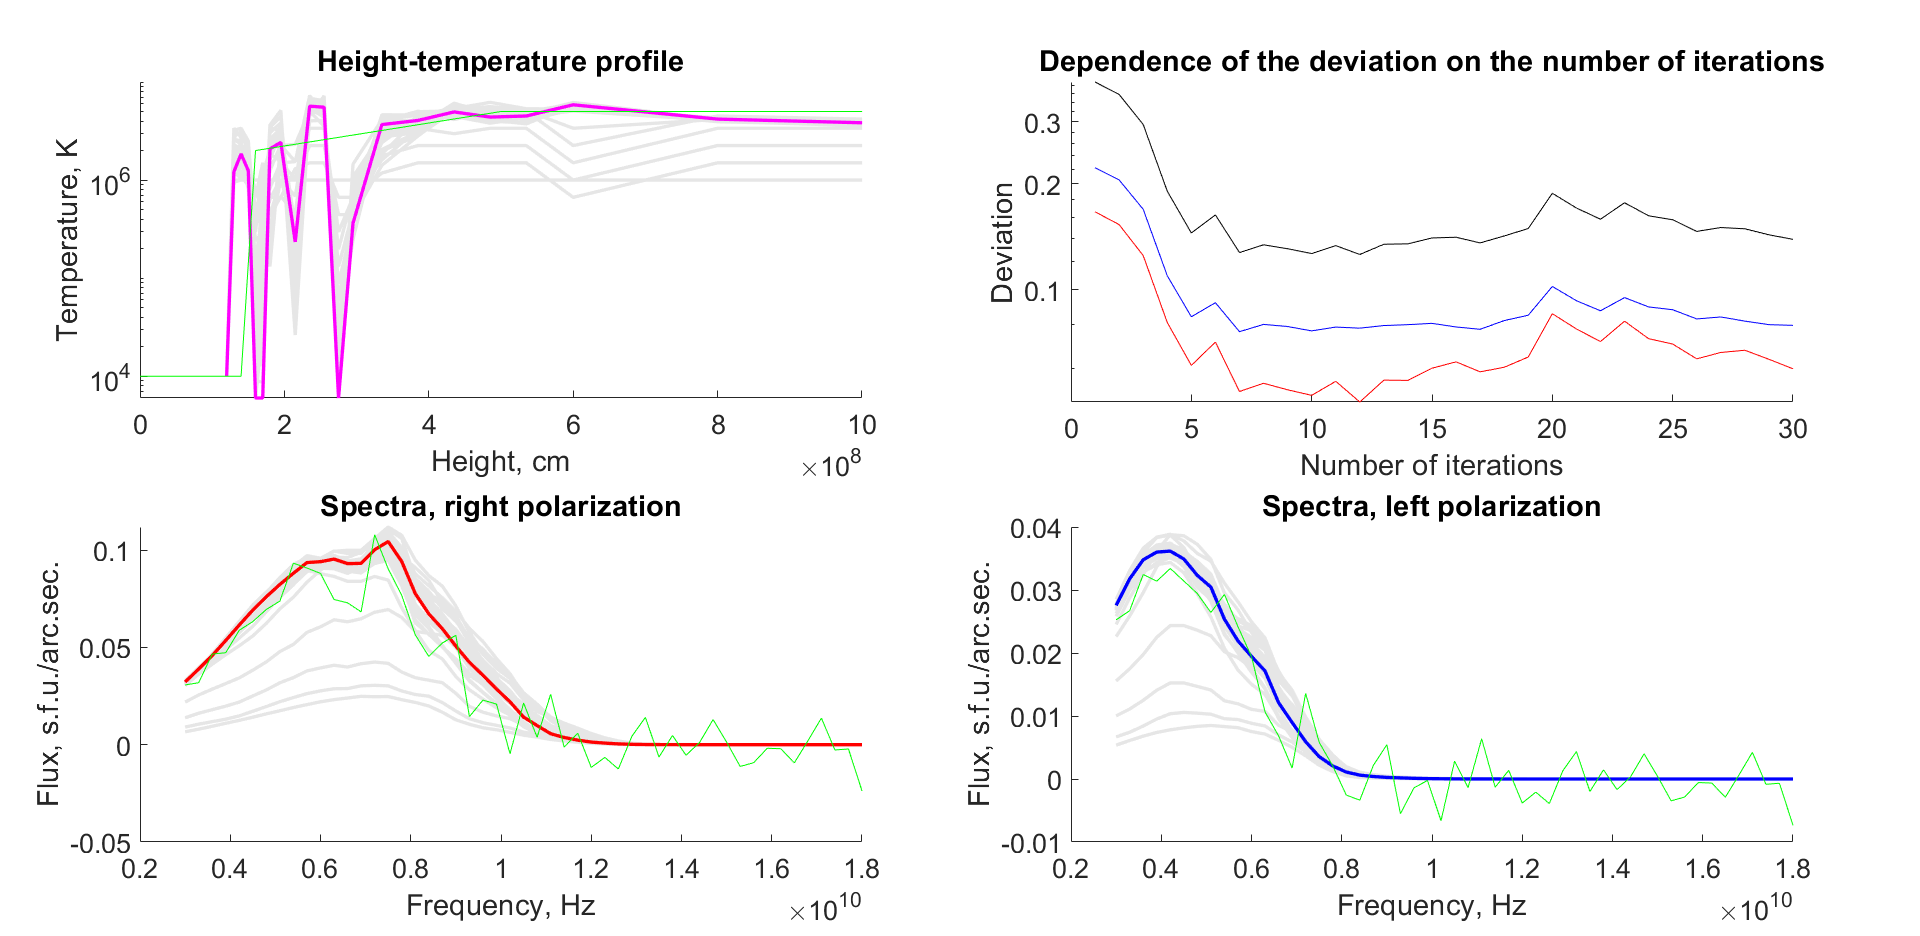
\includegraphics[width=1\linewidth]{AdditiveNoise/10.png}}
\caption{10-процентный аддитивный шум}
\end{figure}
\hfill\break
\hfill\break
\hfill\break
\hfill\break
\hfill\break
\hfill\break
\hfill\break
Уже с 5 процентов начинаются сильные отклонения профиля от тестового в переходной области, в короне профили приблизительно совпадают.
\newpage
\subsection*{Влияние мультипликативного шума}
\begin{figure}[h!]
\center{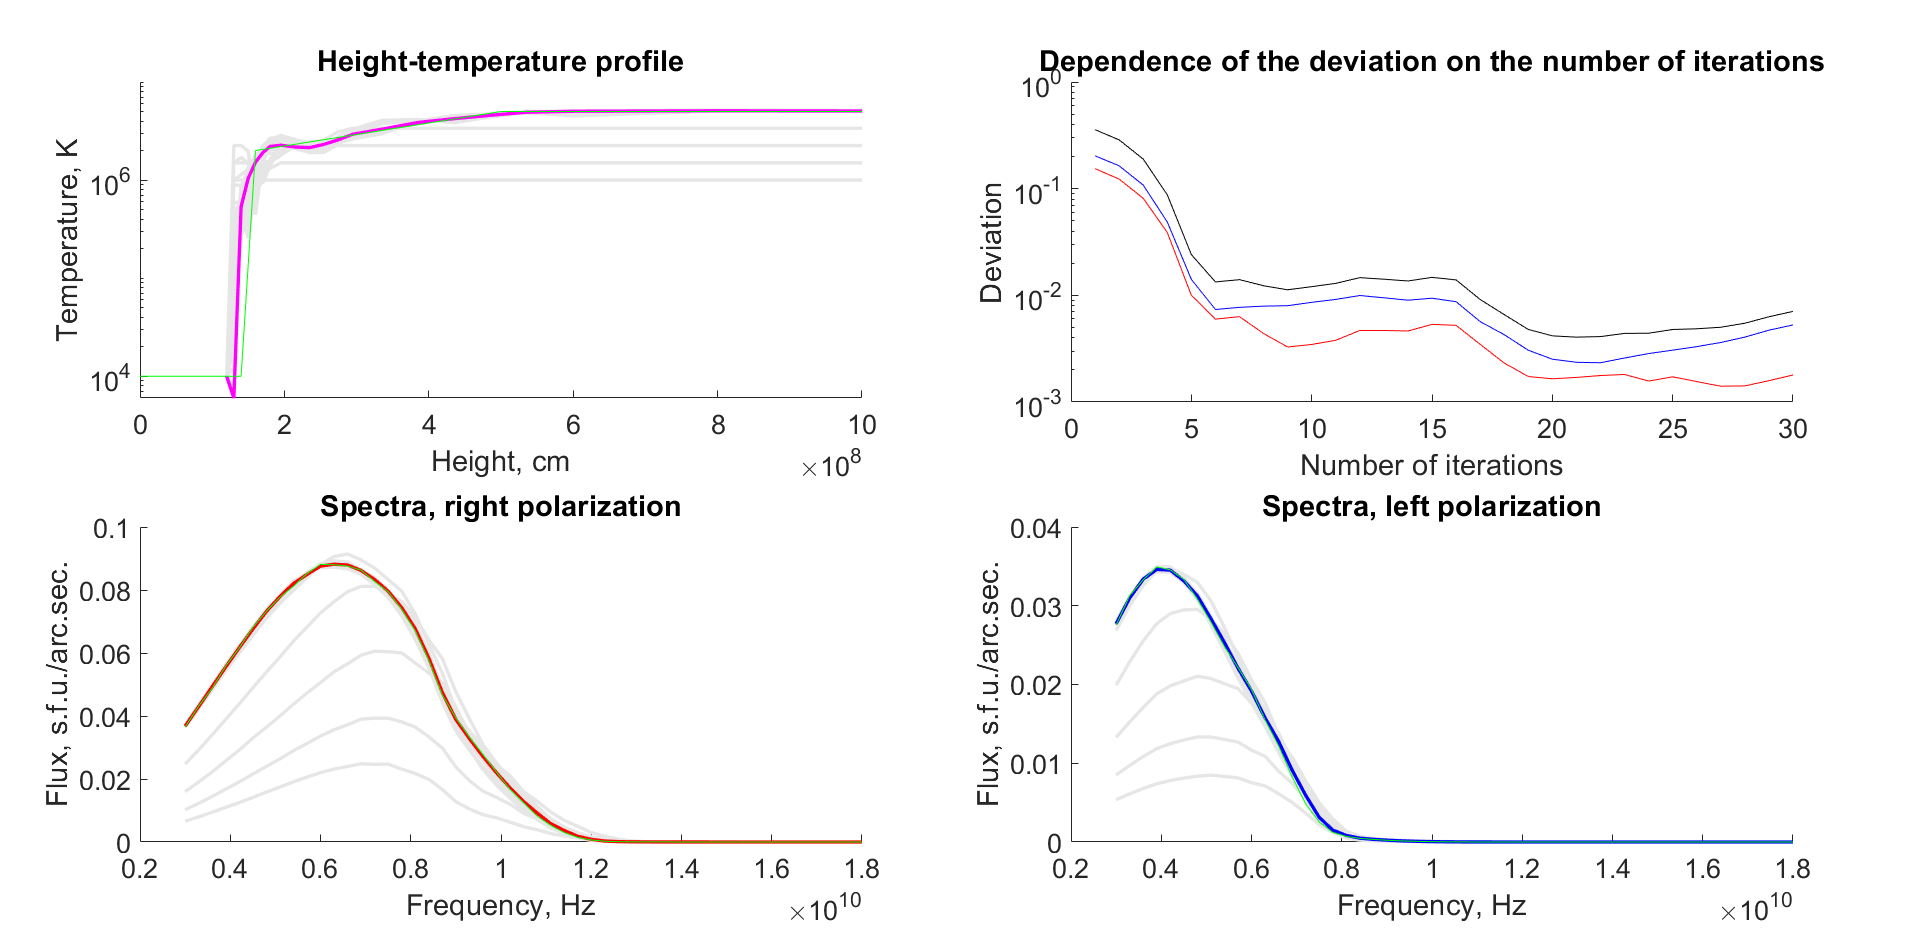
\includegraphics[width=1\linewidth]{MultiplicativeNoise/1.png}}
\caption{1-процентный мультипликативный шум}
\end{figure}
\begin{figure}[h!]
\center{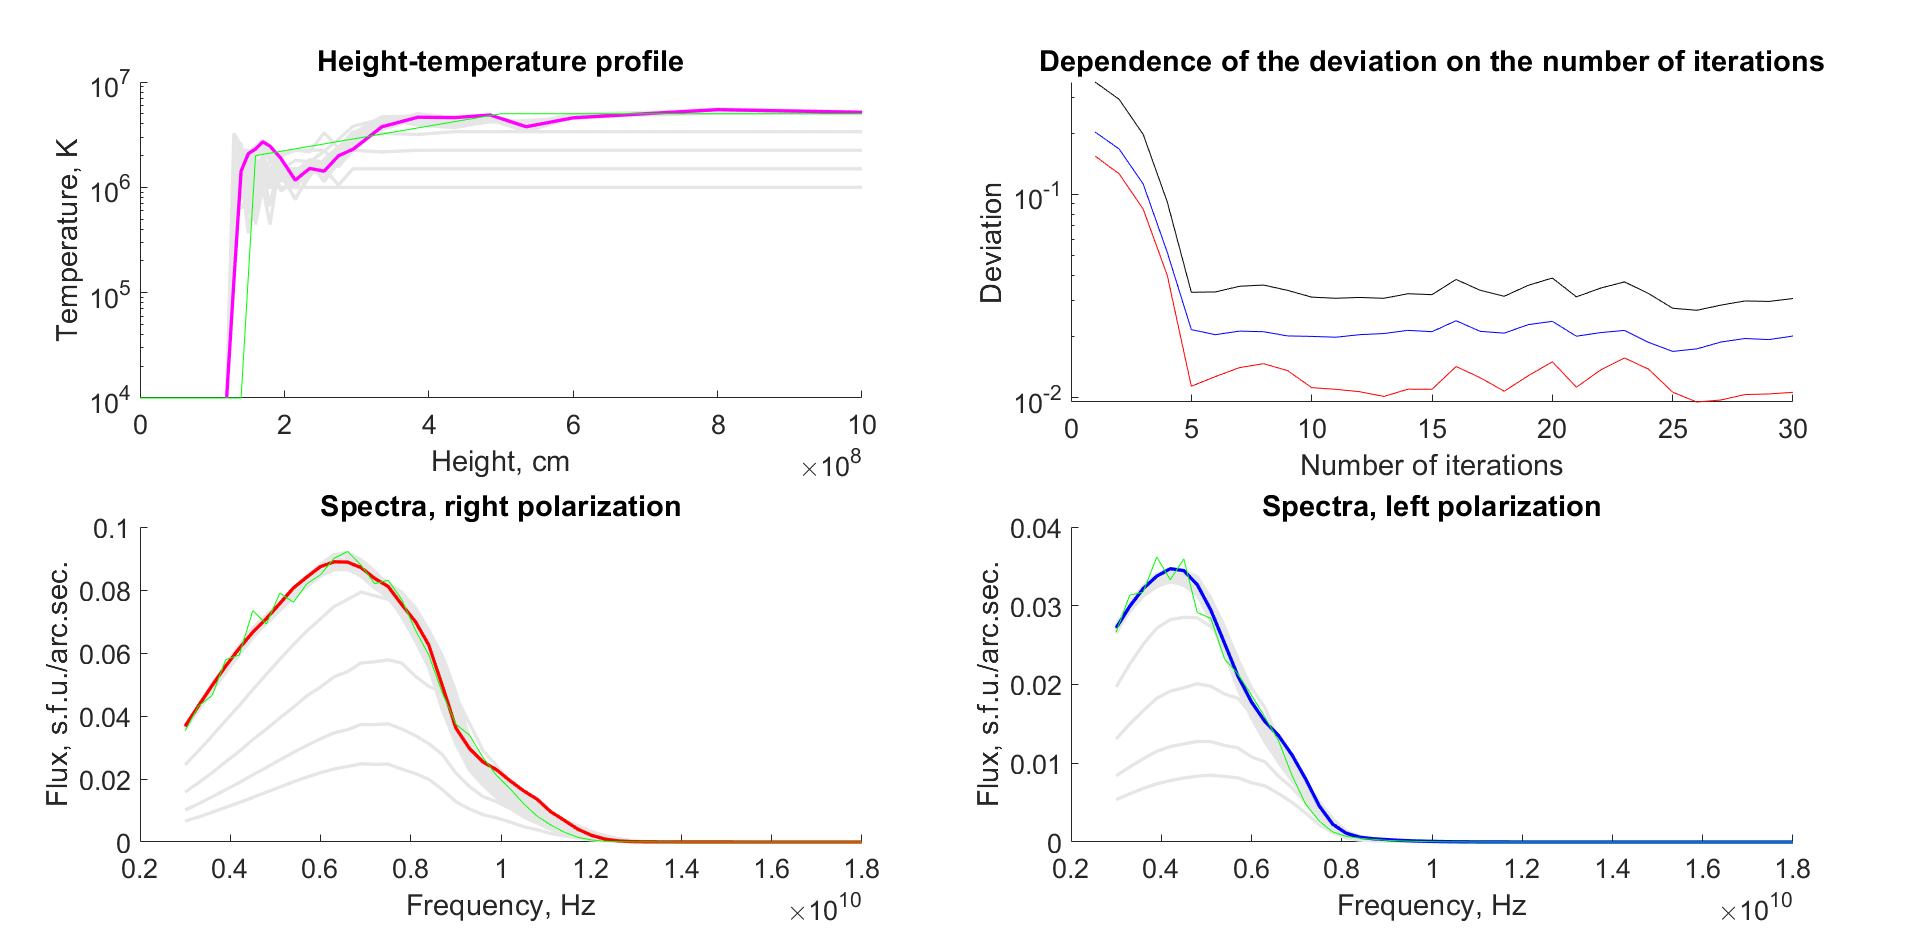
\includegraphics[width=1\linewidth]{MultiplicativeNoise/5.png}}
\caption{5-процентный мультипликативный шум}
\end{figure}
\begin{figure}[h!]
\center{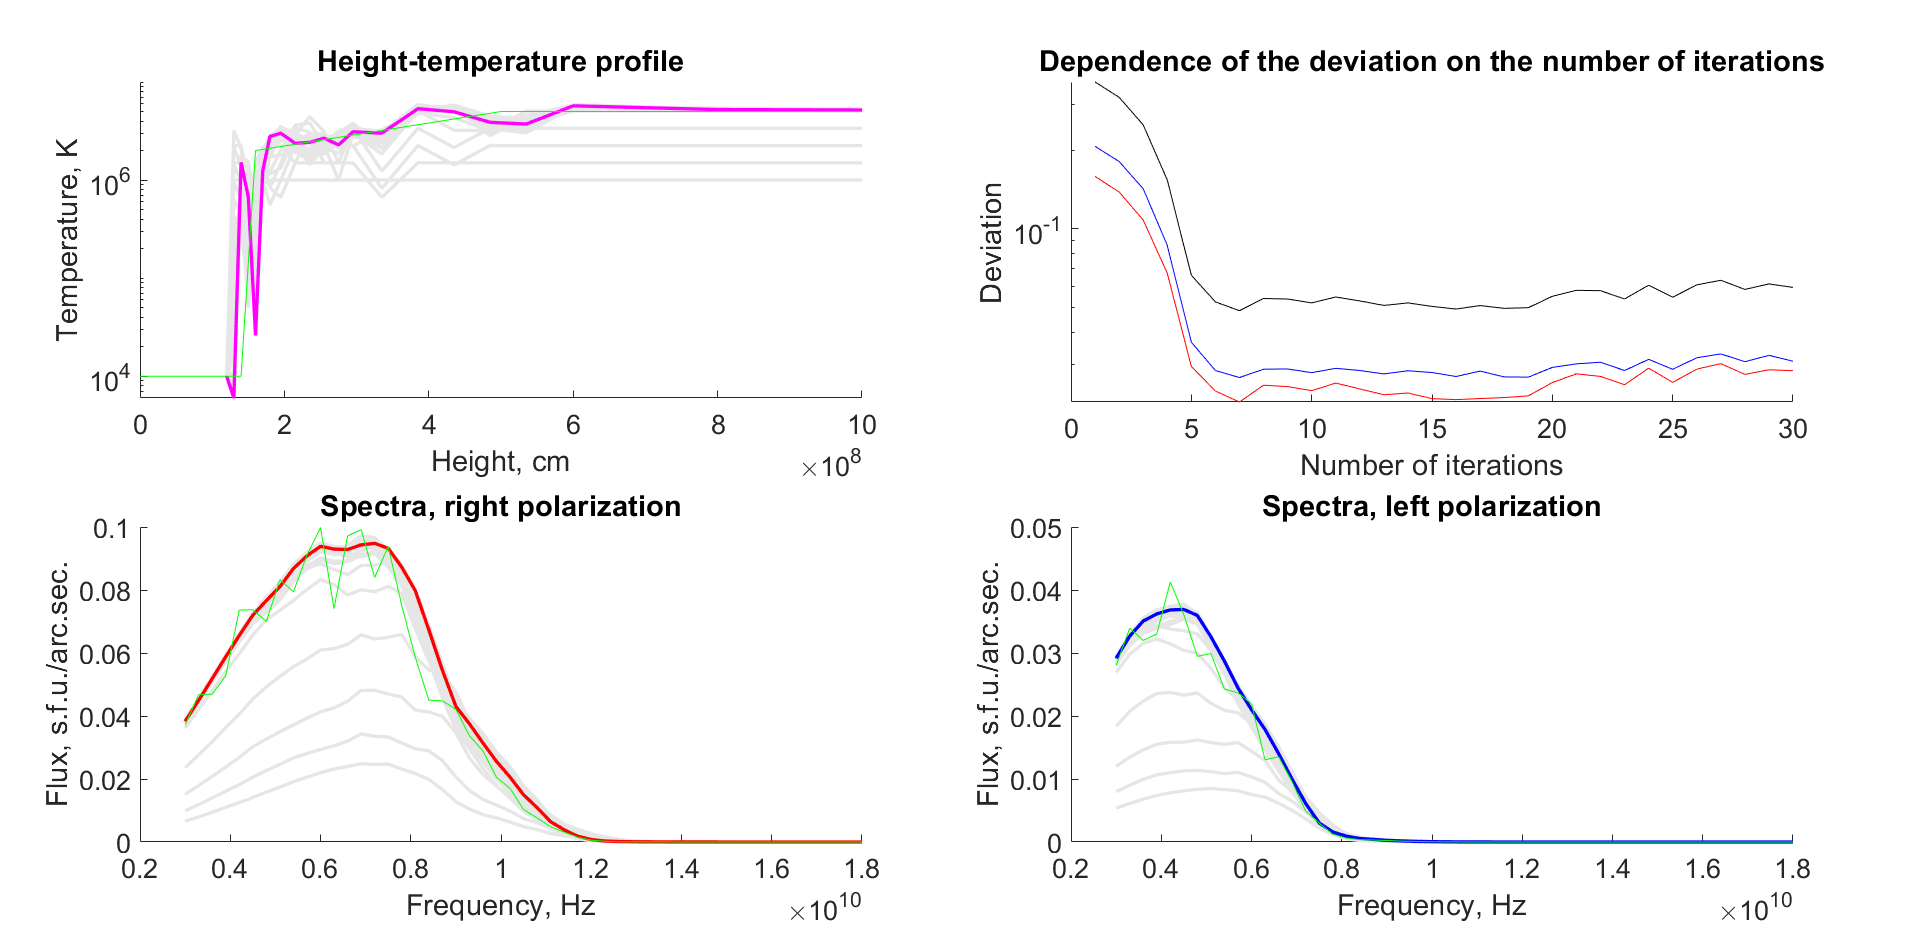
\includegraphics[width=1\linewidth]{MultiplicativeNoise/10.png}}
\caption{10-процентный мультипликативный шум}
\end{figure}
\hfill\break
\hfill\break
\hfill\break
\hfill\break
\hfill\break
\hfill\break
\hfill\break
\hfill\break
Уже с 5 процентов начинаются сильные отклонения профиля от тестового в переходной области, в короне профили приблизительно совпадают.
В целом, искажения профилей и невязка меньше, чем при аддитивном шуме
\end{document}


